\documentclass{acm_proc_article-sp}
\usepackage{url}

\begin{document}

\title{Algorithmic and Economic Aspects of the Internet}
%
% You need the command \numberofauthors to handle the 'placement
% and alignment' of the authors beneath the title.
%
% For aesthetic reasons, we recommend 'three authors at a time'
% i.e. three 'name/affiliation blocks' be placed beneath the title.
%
% NOTE: You are NOT restricted in how many 'rows' of
% "name/affiliations" may appear. We just ask that you restrict
% the number of 'columns' to three.
%
% Because of the available 'opening page real-estate'
% we ask you to refrain from putting more than six authors
% (two rows with three columns) beneath the article title.
% More than six makes the first-page appear very cluttered indeed.
%
% Use the \alignauthor commands to handle the names
% and affiliations for an 'aesthetic maximum' of six authors.
% Add names, affiliations, addresses for
% the seventh etc. author(s) as the argument for the
% \additionalauthors command.
% These 'additional authors' will be output/set for you
% without further effort on your part as the last section in
% the body of your article BEFORE References or any Appendices.

\numberofauthors{2} %  in this sample file, there are a *total*
% of EIGHT authors. SIX appear on the 'first-page' (for formatting
% reasons) and the remaining two appear in the \additionalauthors section.
%
\author{
% You can go ahead and credit any number of authors here,
% e.g. one 'row of three' or two rows (consisting of one row of three
% and a second row of one, two or three).
%
% The command \alignauthor (no curly braces needed) should
% precede each author name, affiliation/snail-mail address and
% e-mail address. Additionally, tag each line of
% affiliation/address with \affaddr, and tag the
% e-mail address with \email.
%
% 1st. author
\alignauthor
Sam Phippen\titlenote{sp9857}\\
       \email{samphippen@googlemail.com}
% 2nd. author
\alignauthor
Luke Murray\titlenote{lm9131}
       \email{lm9131@bris.ac.uk}
}
% There's nothing stopping you putting the seventh, eighth, etc.
% author on the opening page (as the 'third row') but we ask,
% for aesthetic reasons that you place these 'additional authors'
% in the \additional authors block, viz.
% Just remember to make sure that the TOTAL number of authors
% is the number that will appear on the first page PLUS the
% number that will appear in the \additionalauthors section.

\maketitle
\begin{abstract}

For the assignment we attempted to implement the Adaptive
Aggressive\cite{Vytellingum:AA} trading agent strategy. Even with corrections
emailed by D. Cliff we found that our strategy does not trade as efficiently as
is implied in other background research\cite{DC:dominate}. In this paper we've
done a comparative analysis of the existing trading agents provided in BSE,
along with our implementation. We have also performed a post mortem analysis as
to why we believe that our trader is not trading as efficiently as expected.

We had initially set our sights on taking an implementation of AA and trying to
improve upon it, with a view to building something new and potentially more
effective, however, having found ourselves in a position where the agent is
nowhere near as effective as we expected, this was not a good springboard for
extension.

\end{abstract}

\section{Analysis of our agent with existing traders}

\subsection {Many versus many tests} For the analysis we started with a many
versus many test of our implementation versus each of the agents provided with
BSE. In this experiment we used the stepped supply and demand schedule provided
with an early version of the Bristol Stock Exchange, with three distinct time
periods, the first having prices in the range 10-190, the second in the range
200-300 and the third having prices in the same range as the first. In the many
versus many test 20 agents of each type were used (10 sellers and 10 buyers),
and the tests with this supply and demand schedule were repeated a total of 25
times.

The table below shows the number of rounds that our agent lost, the mean
difference in profit between the other agent and ours, and the standard
deviation of the difference in profit also.

\begin{center}
  \begin{tabular}{ l | l | l | l }
        Agent Type & Tests lost & $\Delta$ Profit Mean & $\Delta$ Profit StDev \\\hline
        Giveaway & 24 & 63.84 & 34.16\\
        ZIC & 25 & 75.38 & 36.15\\
        Shaver & 25 & 95.63 & 21.01\\
        Sniper & 25 & 22.67 & 12.78\\
        ZIP & 25 & 97.08 & 41.38\\
  \end{tabular}
\end{center}

In almost all of these cases our agent consistently generated a profit,
however when run against the Shaver agent, an oddity occurred. The agent on
average generated a loss which can be seen on the box plot in figure 1.

\begin{figure}[h!] 
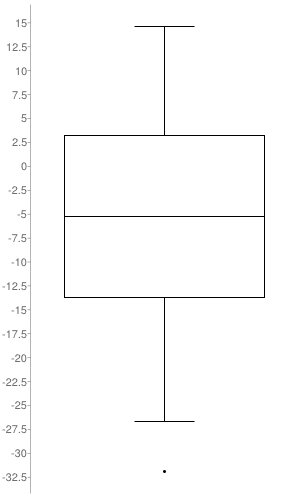
\includegraphics[width=80mm]{box-plot-image.png}

\caption{Box plot of average profits of the 20 AA agents implemented by us in
the many vs many test against shaver agents. Box plot generated from:
http://www.alcula.com/calculators/statistics/box-plot/}
\end{figure}

\subsection{AA v Shaver} One very noticable trend in our analysis is when AA
is pitched against the Shaver algorithm. In all of our experiments where trades
occurred, Shaver made more profit than AA. In this section, we explore the
reasons why Shaver so completely outclasses our implemetation of AA.

Shaver is designed to make "close shave" bids and asks by slightly out-bidding
the best bid on the market. This is similar to how AA's aggressiveness is
supposed to operate; when a bid is placed that out-bids the bot, the price is
adjusted so that the bot out-bids the previous bid in the following round
(unless such a bid would exceed the bot's limit price). This aggressiveness
behaviour increases the chance of a trade and thus increases profit.

We show 3 cases here:
\begin{enumerate}
\item 1 AA bot v. 1 Shaver bot
\item 1 AA bot v. 10 Shaver bots
\item 10 AA bots v. 10 Shaver bots
\end{enumerate}

\subsubsection{1 v 1} No trading occurs in this experiment. In the graphs
below, you can see the shouts made by the bots. The Shaver buyer and seller
traders tend toward the equilibrium price over time but don't manage to reach
it before the market session ends. The AA bot makes very few trades and is
always out-bid / out-asked by Shaver.

\begin{figure}[h!] 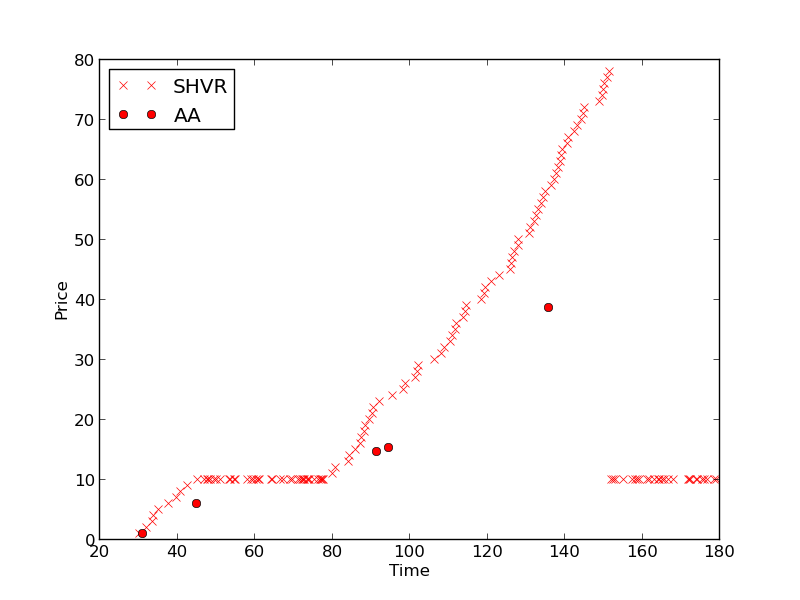
\includegraphics[width=80mm]{SHVR1AA1_180_all_bids.png}
\caption {1 AA versus 1 Shaver. This plot shows the time the time and price of the bids made.}
\end{figure}

\begin{figure}[h!] 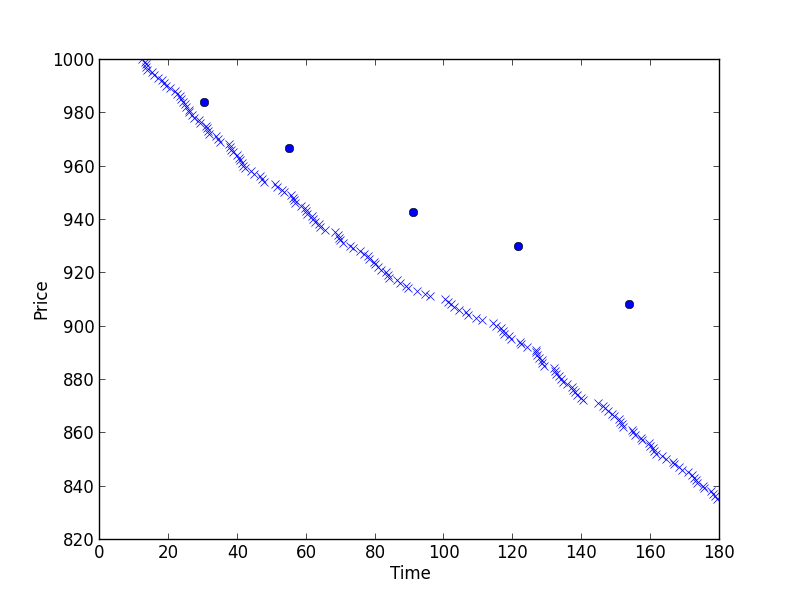
\includegraphics[width=80mm]{SHVR1AA1_180_all_asks.png}
\caption {1 AA versus 1 Shaver. This plot shows the time the time and price of the asks made.}
\end{figure}

\subsubsection{1 v Many} In these experiments, trading starts at around round
90. In the graphs below, we see that the Shaver bots tend towards the
equilibrium much faster than when there was only one bot; this is likely due to
there being 10 Shaver bots which are all trying to out-bid each other. When the
bids and asks converge, the Shaver bots invariably trade with themselves. Our
AA implementation is excluded from trading as it can't adjust its
aggressiveness quickly enough. Not all Shaver bots are engaged in making actual
trades at all times, the horizontal lines of bids / asks on the graphs indicate
that a Shaver bot is placing shouts at its limit price.

\begin{figure}[h!] 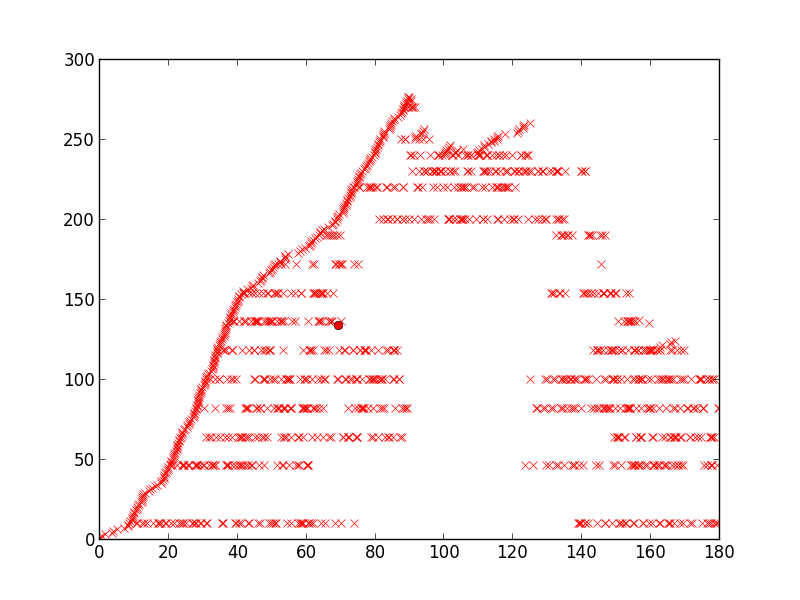
\includegraphics[width=80mm]{SHVR10AA1_180_all_bids.png}
\caption {1 AA versus 10 Shavers. This plot shows the time the time and price of the bids made.}
\end{figure}

\begin{figure}[h!] 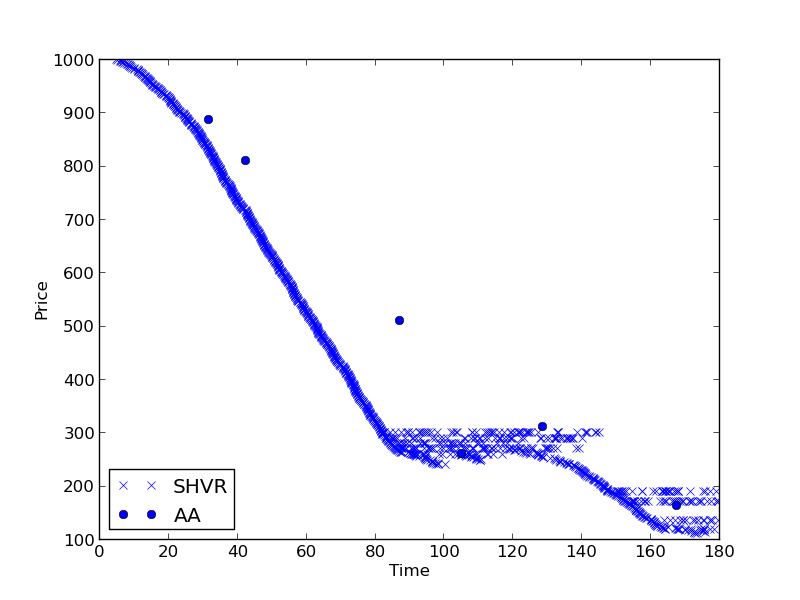
\includegraphics[width=80mm]{SHVR10AA1_180_all_asks.png}
\caption {1 AA versus 10 Shavers. This plot shows the time the time and price of the asks made.}
\end{figure}

Our AA implmentation again demonstrates how it is not tending to the
equilibrium logarithmically as it shold be. Were it functioning correctly, our
AA implementation should have placed bids that were higher (or asks that were
smaller) just after those Shaver placed. This is because AA is designed to
alter its aggressiveness such that it can make competitive shouts in subsequent
rounds, however, it fails to do this. In other words, Adaptive Aggressive is
failing to change it's aggressiveness adaptively.

\subsubsection{Many v Many} Again, trading begins at around round 90. We see
the same pattern as we do in the previous experiment except that AA is making
more bids / asks. On this occasion we see that AA actually manages to make a
few profitable trades between rounds 90 and 140 before being swamped by the
simpler and more effective aggressiveness function of the correctly implemented
Shaver bot. These few trades are more by chance than by design; the dip in bid
price would have intersected with the poorly adapting AA bot allowing AA to
place bids that would be accepted by the seller Shaver traders.

\begin{figure}[h!] 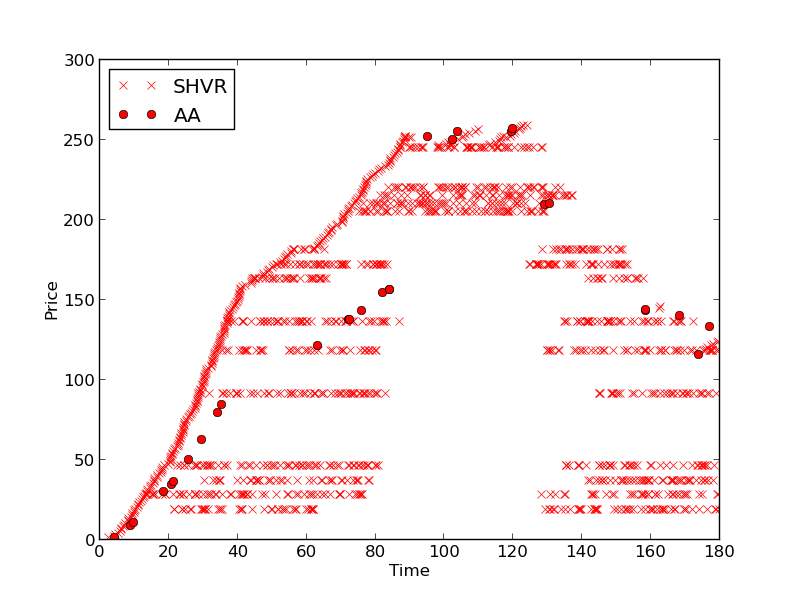
\includegraphics[width=80mm]{SHVR10AA10_180_all_bids.png}
\caption {10 AAs versus 10 Shavers. This plot shows the time the time and price of the bids made.}
\end{figure}

\begin{figure}[h!] 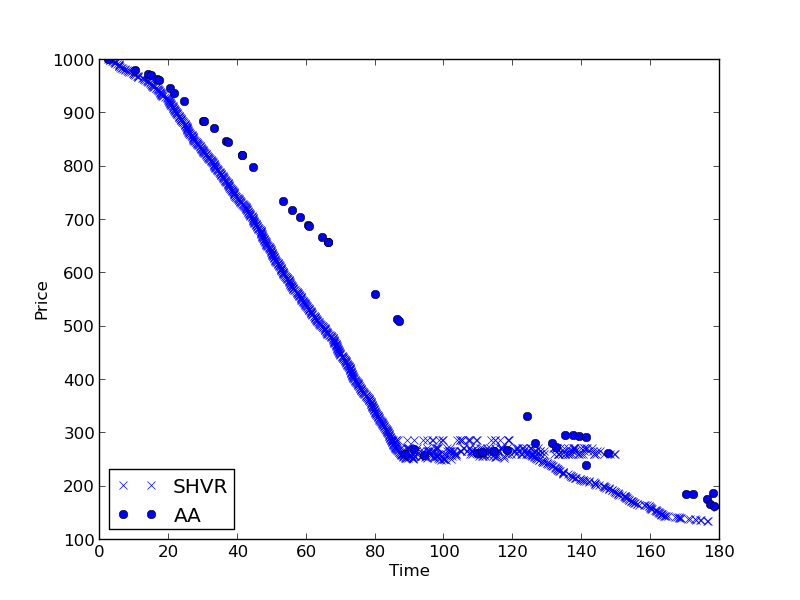
\includegraphics[width=80mm]{SHVR10AA10_180_all_asks.png}
\caption {10 AAs versus 10 Shavers. This plot shows the time the time and price of the asks made.}
\end{figure}

\subsection{1 v 1 tests} Given these initially dismal results, we decided that
a good place to start a detailed analysis would be a 1v1 test with the Giveaway
trader, which is clearly the worst of all the traders within the BSE system.
300 1v1 tests were performed, we used the same schedule as the many versus many
test, with a longer total trading time of 1800. Results where both bots made
zero profit were eliminated, this brought the number of tests included for
analysis down from 300 to 242. Of these tests 103 were won by Giveaway and 139
were won by our agent. The distributions of profit for each agent, as well as
the distribution of differences in profit can be seen in figures 8 and 9.

\begin{figure}[h!] 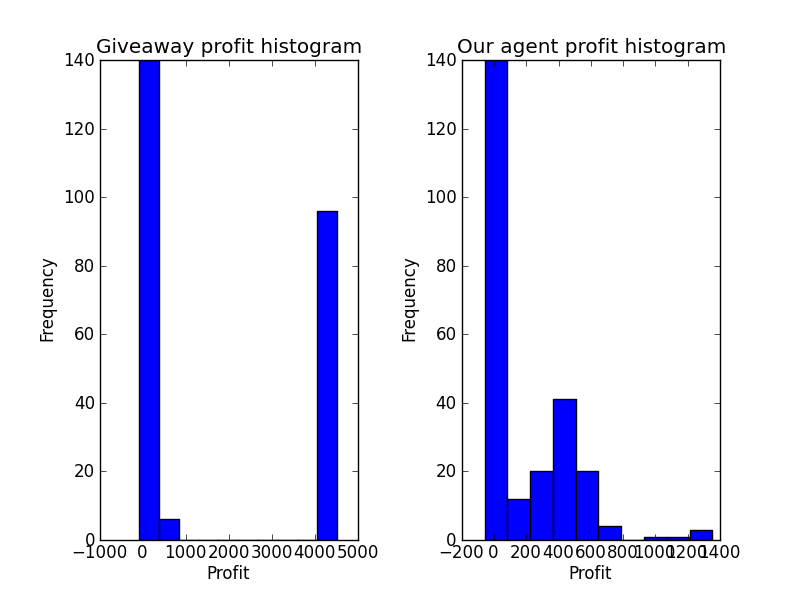
\includegraphics[width=80mm]{giveaway_1_v_1.png}
\caption{Histogram of profit distributions over 300 similar trading runs for
the two bot types used in the 1v1 test. Note axis are different for the two
bots} \end{figure}

\begin{figure}[h!] 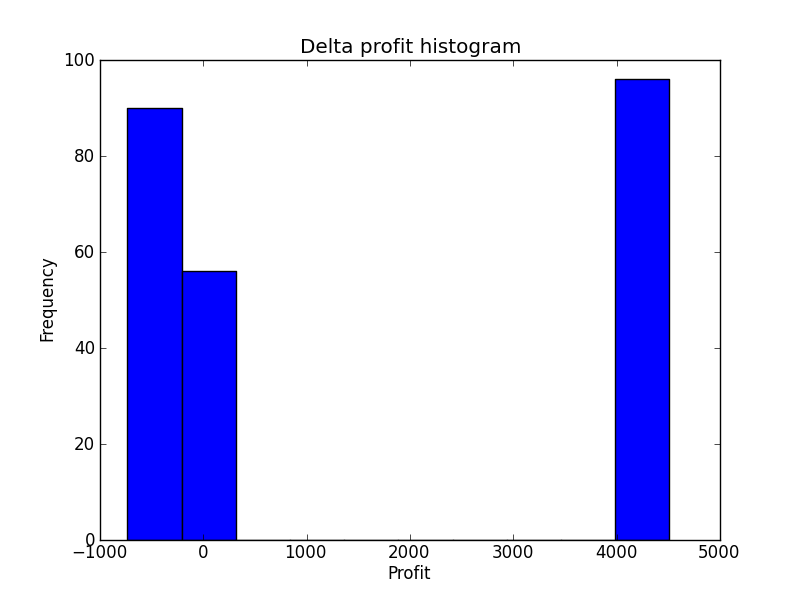
\includegraphics[width=80mm]{giveaway_1_v_1_delta.png}
\caption {Histogram showing the difference between Giveaway and our AA implementation,
positive profit represents cases where Giveaway made more profit than AA}
\end{figure}

\newpage
Upon initially inspecting these graphs we had assumed that our agent should
lose to Giveaway, however we checked the medians of the distributions and noted
that the median profit of the Giveaway agent (1.7) was less than the median
profit (50.0) of our agent. We feel that this difference in profits is the
reason for our agent's overall victory against Giveaway. To determine if the
difference in medians is significant we decided to use the Wilcoxon signed-rank
test\cite{wiki:wilcoxon}. We like this test because:

\begin{enumerate}
\item It makes no assumptions about the underlying
distribution of profit pairs, as we can see from the histogram, these are
nowhere near normally distributed.

\item It handles the fact that the pairs are dependant but the individual runs
are independent.

\item We feel that the assumptions the distribution makes are fulfilled here:
the pairs do come from the same distributions. The pairs have been generated
largely at random by running different tests and collecting results. The data
are obviously ordinal as they are floating amounts of profit.

\end{enumerate}

In order to conduct this test we represented each run as a pair of
$(profit_{giveaway}, profit_{agent})$. The profits in the pair are taken from
the average profit column in the output of running BSE. This means that in
reality the profit values are divided through by two for each agent, as it is
the average of 1 seller and 1 buyer in each case. This does not affect the test
because the change in magnitude is the same for both agents.

The test runs over the difference between the first and second value in the
pair. Our null hypothesis $H0$ is that the median difference of each pair is
zero, with our positive hypothesis $H1$ being that the median difference of
each pair is not zero. We performed the test using scipy's built in Wilcoxon
signed-rank test implementation\cite{scipy:wilcoxon} and the results were
conclusive.  With $p=1.2\times10^{-6}$ we reject $H0$ and conclude
that the difference in medians is significant, as such the difference in
profits generated is statistically significant.

This test was repeated for each of ZIC, Shaver, Sniper and ZIP. In each case,
the results were that, our agent performed worse than the other
agent with our agent having a lower median score and the Wilcoxon test giving
p < 0.01 in each case.

In light of the test against Giveaway it is  worth noting the spike at a profit
of around ~4000 in figure 9.  These occasions correspond to Giveaway making
4000 more profit than our agent. A quick analysis of the data indicates that
nearly all of these occur when our agent issues no trades (zero balance at the
end of trading). As such we concluded that for whatever reason on these events
(96/242 runs) the conditions never reach the point where our agent starts
trading. This is not unreasonable given the warmup period of the algorithm and
the low number of traders in the system.

\subsection{Experiments with supply and demand schedules}

We wanted to determine under what, if any, supply and demand conditions our
agent could outperform some of the better algorithms in the system. In order to
do this we conducted several experiments with varying supply and demand
schedules listed below. We use n=300 as our number of trials, 1 v 1 tests and a
total time period length of 1800. Initially all tests were performed against
ZIC

\subsubsection{Totally open market}

In this set of trials we used the hard limits of BSE, minimum price of 1 and
maximum price of 1000 for both the supply and demand curves, for the entire
time range, using a drip-poisson timemode with a 30 second replenishment time.
The idea behind this experiment is to gather an understanding as to how our
agent performs in a totally unconstrained environment.

The results of this experiment are fairly clear with 164 trials containing
non-zero trading and ZIC winning 115 of these with a median profit of 26973.0
versus a median profit of 0 for our agent the Wilcoxon test shows a clear
statisitical edge for ZIC (p < 0.01).

\subsubsection{Massive financial crash}

In this test we start with a fairly stable market with the price ranging
between 600 and 700. We then intentionally very rapidly crash the market by
dropping the price range to 1-100 for a short range of time before slowly
ramping the price back up.  Refer to figure 10 for the ask and bid orders
issued in one of the 300 example runs.

The rationale behind this is the fact that our agent tracks the equilibrium price
with some accuracy, and as such may be able to more efficiently issue a trade
than ZIC, which is placing its trades at random within the limit prices it has
been given.

In these conditions it is of course extremely difficult for any agent to act
within the market. We have also included a graph of our agent's equilibrium
estimator, this shows that the estimate does a pretty good job keeping up with
the extreme turbulence within the market.

In this experiment all 300 trials had cases where trading occurs. Of these 189
were lost by our agent, however, the medians had a significantly smaller
difference (ZIC 739.47, our agents 519.072136). Whilst this still represents a
statistically significant advantage (p < 0.01 Wilcoxon) for ZIC, it raises an
interesting case where the performance of our agent is significantly improved.
This lead us to our next experiment, which was to effectively repeatedly crash
and restore the market, causing an extremely high volatility.

\begin{figure}[h!] 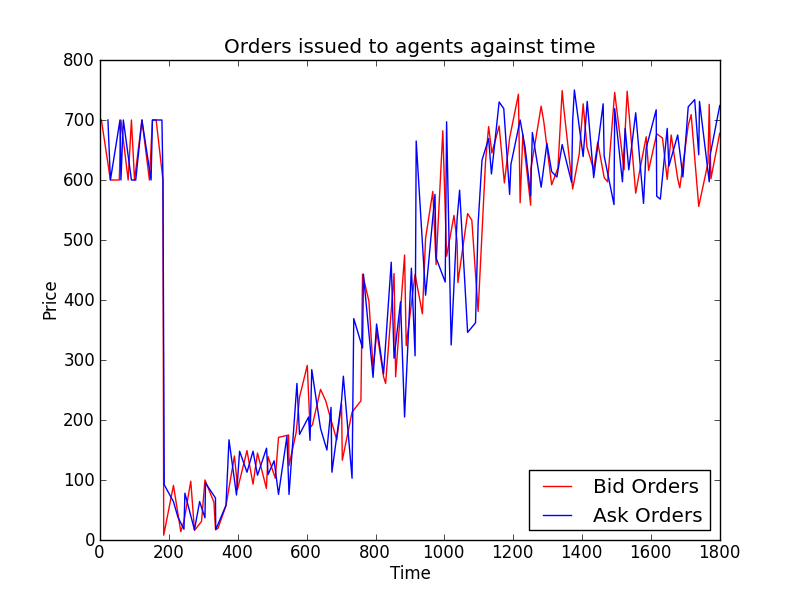
\includegraphics[width=80mm]{crash.png} \caption{Market
order prices given to both buyers and sellers. Extreme volatility introduced at
t=180 by suddenly crashing the market.} \end{figure}

\begin{figure}[h!]
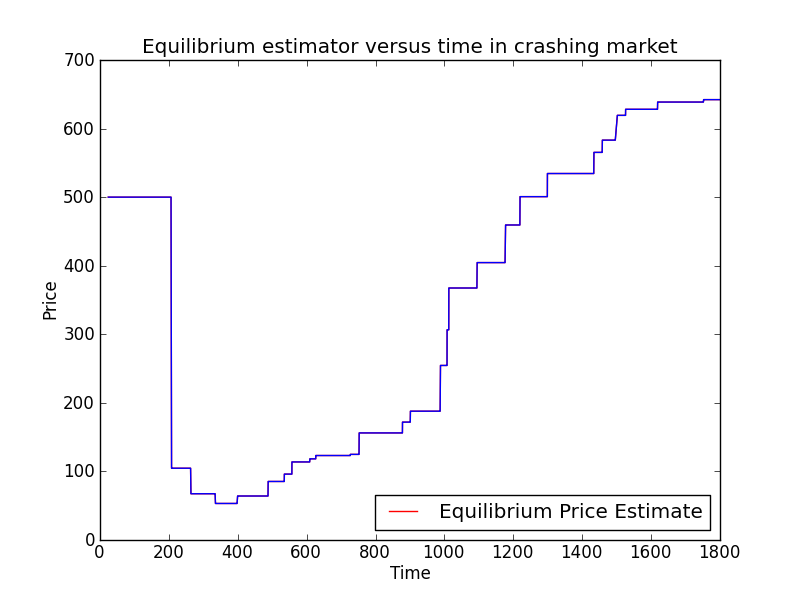
\includegraphics[width=80mm]{crash2.png} \caption{Equilibrium estimate of both
our agent's buyer and seller versions} \end{figure}

\subsubsection{Square wave market}

In this experiment we start with the same inital conditions as the previous
market but we repeatedly change the price ranges from 600-700 and 1-100 and use
the "random" stepmode in an attempt to cause maximum market volatility.

The basic rationale of this experiment is that our agent performed better in
the volatile conditions of the previous experiment, but still performed worse
than ZIC. We wanted to see if this edge case might cause best case behaviour in
our agent. In figure 12 we have provided an example of what the orders placed
look like.

\begin{figure}[h!] 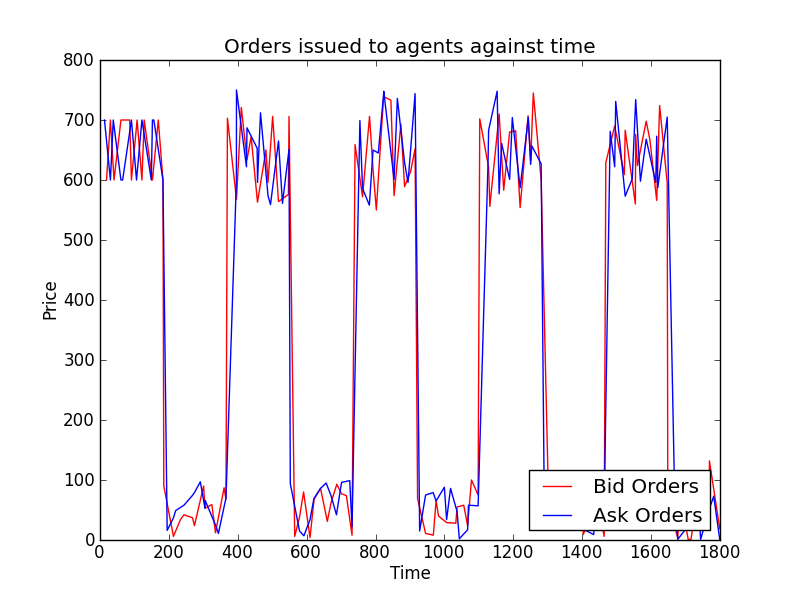
\includegraphics[width=80mm]{squarewave.png} \caption{Market
order prices given to both buyers and sellers. Periodic volatility introduced
every 180 timesteps} \end{figure}

Unfortunately this experiment did not produce the expected results, with ZIC
managing to extract a much higher median profit than in the previous experiment
(1535.48). Our agent also extracted a slightly higher profit than the previous
experiment (median 703.82).

From these analysis we basically conclude that whilst our bot trades more
efficiently than giveaway it does not trade more efficiently than ZIC in both
stable and extremely unstable market conditions. Whilst this is disappointing
we find an obvious reason for this result: our implementation, which attempts
to follow the maths in the original Vytelingum\cite{Vytellingum:AA} paper,
there are flaws in the implementation which cause it not to trade anywhere near
as efficiently as expected, causing it to essentially fail to trade.

Our implementation also seems to issue significantly fewer trades than would be
expected
--luke expand this

\section{Analysing the other traders}

In this section we wanted to analyse the ZIP agent against all the others.
Based on the COMSM2006\cite{cliff:lecture} lecture about trading agents.
Specifically the lecture references an article written by D. Cliff which is
meant to show a case where ZIC traders will not converge to the equilibrium
price of the market\cite{cliff:minimalint}.

%
% The following two commands are all you need in the initial runs of your .tex
% file to produce the bibliography for the citations in your paper.
\bibliographystyle{acm} \bibliography{paper}  % sigproc.bib is the name of
% You must have a proper ".bib" file and remember to run: latex bibtex latex
% latex to resolve all references
%
% ACM needs 'a single self-contained file'!
%
%APPENDICES are optional \balancecolumns
\appendix \end{document}
